\section{Аналитические раздел}

\subsection{Схема модели в терминах СМО}

В процессе взаимодействия клиентов с информационным центром возможны:

\begin{itemize}
	\item режим нормального обслуживания (клиент выбирает одного из свободных операторов, но предпочитает того, у которого меньше номер);
	\item режим отказа (все операторы заняты).
\end{itemize}
Согласно условию, время обработки заявки оператором подчиняется закону равномерного распределения, компьютер же выполняет каждую обработку за фиксированное время.

Эндогенные переменные:

\begin{itemize}
	\item время обработки заданий $i$-ым оператором ($i = \overline{0;2}$);
	\item время решения задания на $j$-ом компьютере ($j = \overline{0;1}$).
\end{itemize}

Экзогенные переменные:

\begin{itemize}
	\item $n_0 =$ числу обслуженных клиентов;
	\item $n_1 =$ числу клиентов получивших отказ.
\end{itemize}

Уравнения модели – $\Large \frac{n_1}{n_0+n_1}$ (вероятность отказа).

За единицу дискретного времени выбрана 0.01 минуты.

\subsection{Результаты программы}


На рисунке \ref{fig:r2} редставлен результат работы программы при различных параметрах.

\begin{figure}[ht!]
	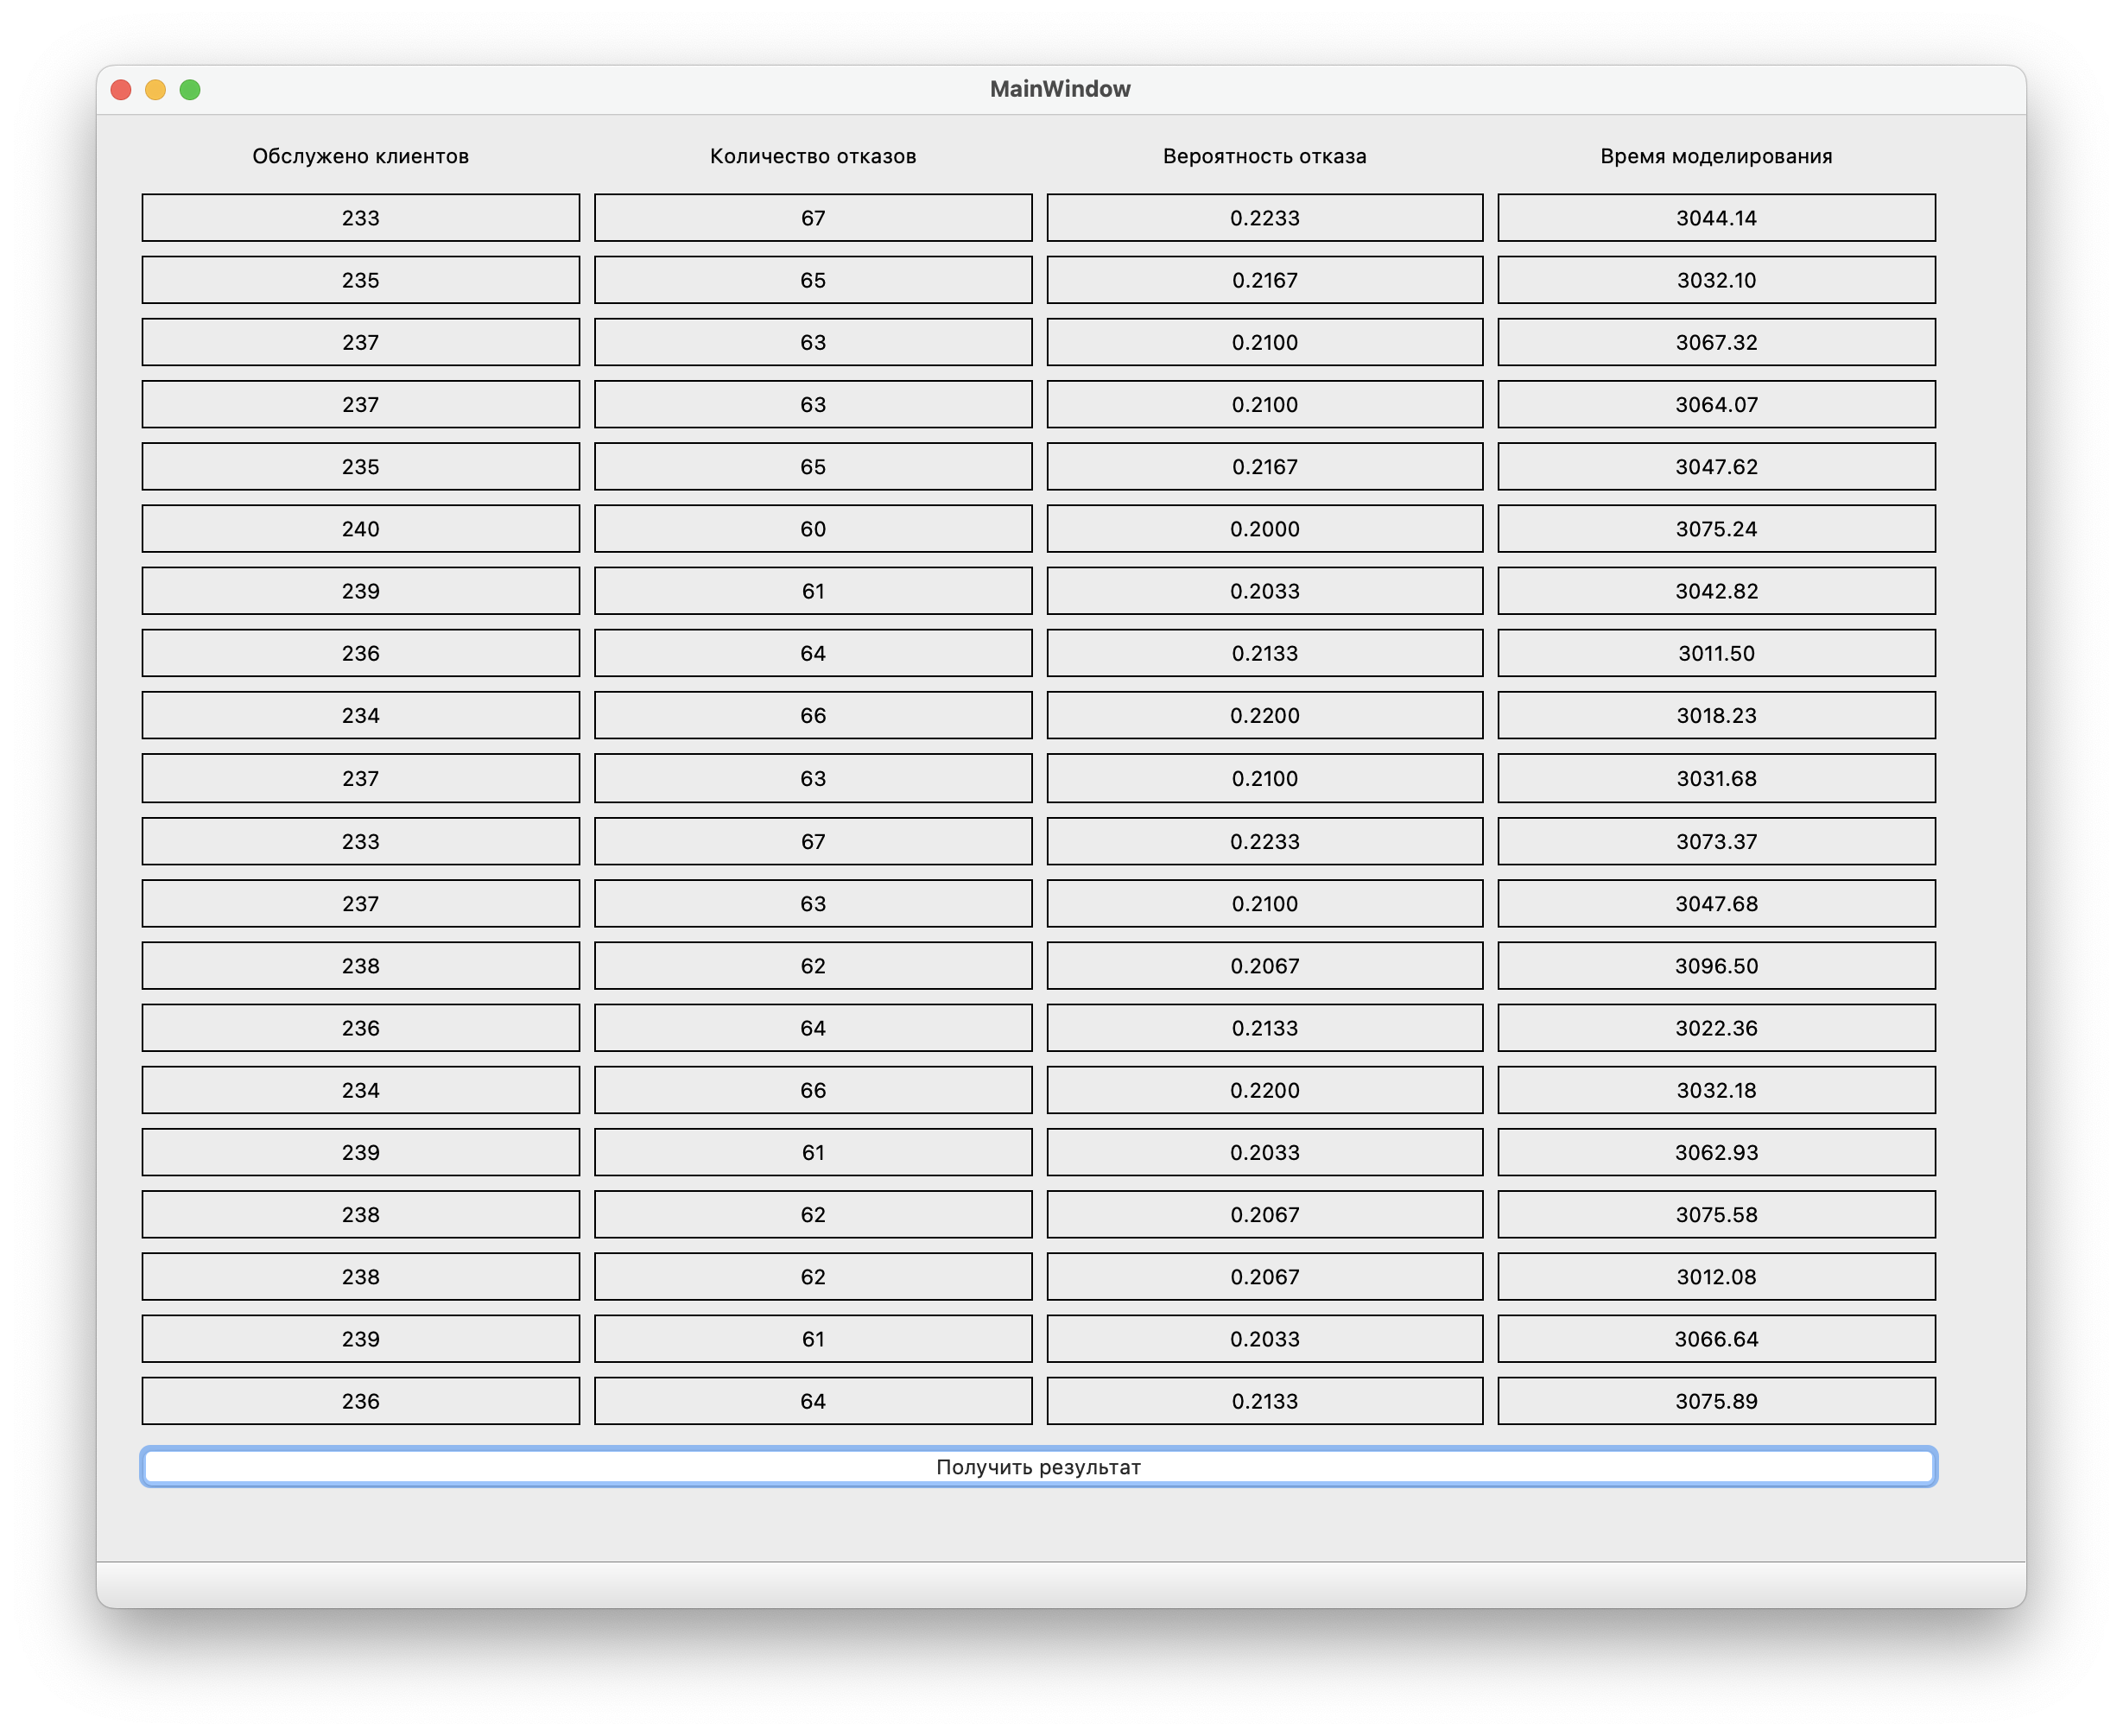
\includegraphics[width=0.75\linewidth]{assets/images/lab-5.png}
	\caption{Результат работы прораммы}
	\label{fig:r2}
\end{figure}